\chapter{Introducción a la teoría de cuerdas}

En primer lugar, veremos como describir una cuerda clásicamente en relatividad especial.
Tras esto, cuantizaremos la cuerda en la gauge del cono de luz, obteniendo una descripción de la cuerda bosónica.
Como procedimiento alternativo, introduciremos la integral de camino.
Por último, comentaremos la dualidad T, que aparece al haber dimensiones compactas.

En este trabajo, seguiremos los siguientes convenios:
\begin{itemize}
  \item La  componente temporal de la métrica de Minkowski tiene signo menos y las componentes espaciales signo más.
  \item El número de dimensiones espacio-temporales es $d$ y el número de dimensiones espaciales no compactas $D$.
  \item Los índices latinos denotan las componentes espaciales de un tensor y toman valores de $1$ a $d-1$, mientras que los índices griegos
  incluyen también la componente temporal y toman valores de $0$ a $d-1$. 
  \item Si hay índices repetidos arriba y abajo en una expresión tensorial, se aplica el convenio de la suma de Einstein.
  \item El determinante de un tensor con componentes $G_{\mu\nu}$, como puede ser la métrica, se denota por $G$.
  \item Emplearemos unidades en las cuales $\hbar = 1$ y $c=1$.
\end{itemize}

\section{La cuerda relativista}

La teoría de cuerdas parte de considerar que las entidades fundamentales son cuerdas
en vez de partículas. 

La trayectoria $\mathbf x(t)$ de una partícula satisface que su acción $S$ es un extremal.
Informalmente, esto significa que la variación de la acción a primer orden es nula bajo
variaciones pequeñas de la trayectoria, supuestas fijas las posiciones iniciales y finales.
La acción de una partícula libre relativista es
\begin{equation}
  S=-m\int dt \sqrt{1-\dot {\vec{x}} \cdot \dot {\vec{x}}},
\end{equation}
donde $\dot x = \dv{x}{t}$.

Para que en la acción aparezca el tiempo y la posición en igualdad de condiciones,
parametrizamos el tiempo y la posición por el tiempo propio $\tau$. 
El tiempo propio es el tiempo que mediría un reloj que se moviese con la partícula.
Con esta transformación, la acción es
\begin{equation}
 S = -m\int d\tau \sqrt{-\dv{x^\mu}{\tau}\dv{x^\nu}{\tau}\eta_{\mu\nu}}=-m\int d\tau,
\end{equation}
donde $x^\mu(\tau)=(t(\tau),\mathbf x(\tau))$ es el cuadrivector posición y $\eta_{\mu\nu}$ la
métrica de Minkowski.

\begin{wrapfigure}{r}{0.3\textwidth}
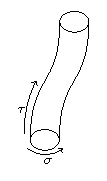
\includegraphics[width=0.2\textwidth]{string.pdf}
 \caption{Trayectoria de una cuerda cerrada.}                   
\end{wrapfigure}
Generalizaremos la acción de una partícula libre a una cuerda libre en $d$ dimensiones espacio-temporales.
Una cuerda está parametrizada por una variable temporal $\tau$ y una variable espacial $\sigma$, adimensional.
De forma más compacta, $(\sigma^1,\sigma^2)=(\tau,\sigma)$. 
La trayectoria de la cuerda en el espacio-tiempo genera un superficie llamada \emph{worldsheet}.
Las coordenadas en la worldsheet $(\tau,\sigma)$ determinan un punto del espacio-tiempo $X^\mu$, también llamado
espacio \emph{target} para evitar confusión.
En este trabajo, consideraremos solo cuerdas cerradas. 
Si la cuerda tiene periodicidad $2\pi$, $X^\mu(\tau,\sigma)=X^\mu(\tau,\sigma+2\pi)$.

\subsection{Acción de Nambu-Goto}

La acción de una partícula es proporcional a la longitud de su línea de universo.
De forma análoga, la acción de una cuerda debería ser proporcional al área de la
worldsheet.
Para poder medir el área, es necesario definir una métrica $\gamma_{\alpha\beta}$ en la worldsheet (en este caso, $\alpha$ y $\beta$ 
toman solo los valores $1$ y $2$).
La forma natural de definir una métrica en una superficie, a partir de la métrica del espacio que
contiene a la superficie, es mediante el concepto de \emph{pull-back}.
En este caso, la métrica en la worldsheet es el pull-back de la métrica de Minkowski
\begin{equation}
  \gamma_{ab}=\pdv{X^\mu}{\sigma^\alpha}\pdv{X^\nu}{\sigma^\beta}\eta_{\mu\nu}.
\end{equation}

La propiedad esencial de la métrica $\gamma_{\alpha\beta}$ es que la distancia entre dos puntos próximos 
coincide con la calculada con la métrica $\eta_{\mu\nu}$, ya que
\begin{equation}
  g_{\mu\nu}(X(\sigma)) dX^\mu(\sigma)dX^\nu(\sigma) = \gamma_{\alpha\beta} d\sigma^\alpha d\sigma^\beta.
\end{equation}

El área de la worldsheet es $\int d^2\sigma \sqrt{-\det\gamma}$, por lo que la acción, llamada de Nambu-Goto, es
\begin{equation}
  S_{NG}=-T\int d^2\sigma \sqrt{-\det\gamma}.
\end{equation}

El parámetro $T$ se corresponde con la tensión de la cuerda y se puede expresar como
\begin{equation}
  T=\frac{1}{2\pi\alpha'},
\end{equation}
donde $\alpha'$ es la pendiente de Regge.
Como $\alpha'$ tiene dimensiones de longitud al cuadrado, define una longitud característica
de la cuerda, $l_s=\sqrt{\alpha'}$.

\subsection{Acción de Polyakov}

A la hora de cuantizar la teoría, la raíz cuadrada es problemática, por lo que se introduce
un campo tensorial $h$ definido sobre la worldsheet en la llamada acción de Polyakov
\begin{equation}
  S_P=-\frac{1}{4\pi\alpha'}\int d^2\sigma  \sqrt{-h}h^{\alpha\beta}\partial_\alpha X^\mu \partial_\beta X_\mu.
\end{equation}

Este campo $h$ se comporta como una métrica en dos dimensiones y queda fijado por las
ecuaciones de movimiento
\begin{equation}
  h_{\alpha\beta}=2f(\sigma)\partial_\alpha X^\mu \partial_\beta X_\mu
\end{equation}
donde $f(\sigma)$ es una función cualquiera. La libertad de poder escoger $f(\sigma)$
es una simetría gauge.

Una simetría es una transformación que deja invariante la acción. 
Si la transformación depende de las coordenadas, se dice que es una simetría gauge. 
Por ejemplo, el campo eléctrico se obtiene a partir de el potencial escalar $\phi$ y
el potencial vector $\mathbf A$ como $\mathbf E = -\nabla \phi - \partial_t \mathbf A$.
Si hacemos las transformaciones $\phi \to \phi + \partial_t \xi(t,\mathbf x)$ y 
$\mathbf A \to \mathbf A + \nabla \xi(t,\mathbf x)$, el campo eléctrico no cambia.
Visto de otro modo, la simetría gauge expresa una redundancia en la descripción del sistema,  
puesto que varias configuraciones distintas corresponden al mismo estado físico.
La acción de Polyakov presenta dos simetrías gauge en la worldsheet que nos interesan:
\begin{itemize}
  \item La simetría bajo reparametrizaciones, dada por un cambio de coordenadas de la worldsheet $\sigma^\alpha \to \tilde \sigma^\alpha$. 
  \item La simetría de Weyl, que se obstiene al transformar la métrica de la worldsheet de acuerdo 
    a
    \begin{equation}
      h_{\alpha\beta}(\sigma) \to \Omega^2(\sigma) h_{\alpha\beta}(\sigma).
    \end{equation}
    Intuitivamente, una transformación Weyl corresponde a un cambio local de escala que mantiene
    deja invariante la medida de ángulos.
\end{itemize}



\section{Cuantización}

Debido a la simetría gauge de la teoría, la cuantización no es directa.
Hay grados de libertad que no son físicos y en algún momento hemos de deshacernos de ellos.
Para obtener directamente una teoría unitaria, cuantizamos solo los grados de libertad 
físicos, buscando primero las soluciones clásicas. 
Como contrapartida, perdemos la invariancia de Lorentz explícita.

Definimos las coordenadas en el cono de luz
\begin{equation}
  \sigma^\pm=\tau\pm\sigma
\end{equation}

\begin{equation}
  X^\pm=\frac{1}{\sqrt 2} (X^0 \pm X^{d-1}).
\end{equation}

Gracias a la simetría gauge, fijamos la métrica en la worldsheet $h_{\alpha\beta}=\eta_{\alpha\beta}$, de forma que 
la acción de Polyakov es
\begin{equation}
  S = -\frac{1}{4\pi\alpha'} \int d^2\sigma \partial_\alpha X^\mu \partial^\alpha X_\mu,
\end{equation}
que da lugar a la ecuaciones de movimiento de ondas libres
\begin{equation}
  \partial_\alpha \partial^\alpha X^\mu=0.
\end{equation}

La solución general de la ecuación de movimiento se descompone
en una onda moviéndose hacia la izquierda $X^\mu_L$ y otra hacia la derecha $X^\mu_R$,
\begin{equation}
   X^\mu =X^\mu_L(\sigma^+) + X^\mu_R(\sigma^-).
\end{equation}

Teniendo en cuenta la periodicidad en $\sigma$, la expansión de Fourier conduce a
\begin{equation}
  \begin{gathered}
    X^\mu_L=\frac 1 2 x^\mu + \frac 1 2 \alpha' p^\mu \sigma^+ + i\sqrt{\frac{\alpha'}{2}}\sum_{n\neq 0} \frac{1}{n}\bar \alpha^\mu_n e^{-in\sigma^+},\\
    X^\mu_R=\frac 1 2 x^\mu + \frac 1 2 \alpha' p^\mu \sigma^- +i\sqrt{\frac{\alpha'}{2}}\sum_{n\neq 0} \frac{1}{n}\alpha^\mu_n e^{-in\sigma^-}.
  \end{gathered}
\end{equation}
Donde $x^\mu$ y $p^\mu$ se corresponden con la posición y el momento del centro de masas de la cuerda, respectivamente. 
Las coeficientes del desarrollo de Fourier se denotan por $\bar \alpha^\mu_n$ y $\alpha^\mu_n$.
Los factores numéricos, las constante $\alpha'$ y $1/n$ se introducen por comodidad.

En términos de $X^+$, tendríamos
\begin{equation}
   X^+ =X^+_L(\sigma^+) + X^+_R(\sigma^-).
\end{equation}

Debido a la invariancia baja reparametrizaciones, escogemos unas coordenadas de forma que
\begin{equation}
  X^+_L=\frac 1 2 x^+ + \frac 1 2 \alpha' p^+ \sigma^+,
\end{equation}
y
\begin{equation}
  X^+_R=\frac 1 2 x^+ + \frac 1 2 \alpha' p^+ \sigma^+.
\end{equation}

Por tanto, 
\begin{equation}
  X^+ = x^+ + \alpha' p^+ \tau.
\end{equation}
La constante $x^+$ puede eliminarse mediante una traslación en $\tau$.

Con esta elección gauge, la solución $X^-$ que determinada casi por completo.
La ecuación de movimiento para la métrica $h$ se obtiene imponiendo que la variación de la acción
se anule para toda variación de la métrica $\delta h$,
\begin{equation}
  \delta S = \frac{1}{4\pi\alpha'}\int d^2\sigma \delta h^{\alpha\beta}
  \qty(
  \sqrt{-h}\partial_\alpha X^\mu \partial_\beta X_\mu -
  \frac 1 2 \sqrt{-h}h_{\alpha\beta}h^{\rho\sigma} \partial_\rho X^\mu \partial_\sigma X_\mu).
\end{equation}
Como habíamos elegido $h_{\alpha\beta}=\eta_{\mu\nu}$, la ecuación de movimiento es
\begin{equation}
  \partial_\alpha X^\mu \partial_\beta X_\mu - \frac 1 2 \eta_{\alpha\beta} \eta^{\sigma\rho} 
  \partial_\rho X^\mu  \partial_\sigma X_\mu = 0.
\end{equation}

En las coordenadas del cono de luz, esto se traduce en
\begin{equation}
  \partial_+ X^\mu \partial_+ X_\mu = \partial_- X^\mu \partial_- X_\mu = 0.
  \label{eq:lig}
\end{equation}

Haciendo la descomposición de la solución $X^-$,
\begin{equation}
  X^-=X^-_L(\sigma^+)+X^-_R(\sigma^-),
\end{equation}
la ecuación \ref{eq:lig} conduce a 
\begin{equation}
  -2\partial_+ X^+ \partial_+ X^- + \sum_{i=1}^{d-2} \partial_+ X^i \partial_+ X^i = 0.
\end{equation}

Sustituyendo el la expresión de $X^+$,
\begin{align}
  \partial_+ X_L^- = \frac{1}{\alpha'p^+}\sum_{i=1}^{d-2} \partial_+ X^i \partial_+ X^i, \label{eq:lig1}\\
  \partial_- X_R^- = \frac{1}{\alpha'p^+}\sum_{i=1}^{d-2} \partial_- X^i \partial_- X^i. \label{eq:lig2}
\end{align}
En el desarrollo de Fourier
\begin{equation}
  \begin{gathered}
    X^-_L(\sigma^+)=\frac 1 2 x^- + \frac 1 2 \alpha' p^- \sigma^+ + i\sqrt{\frac{ \alpha'}{ 2}}
    \sum_{n\neq0} \frac 1 n \bar{\alpha}^-_n e^{-in\sigma^+} \\                             
    X^-_R(\sigma^+)=\frac 1 2 x^- + \frac 1 2 \alpha' p^- \sigma^- + i\sqrt{\frac{ \alpha'}{ 2}}
    \sum_{n\neq0} \frac 1 n \alpha^-_n e^{-in\sigma^-},
  \end{gathered}
\end{equation}
las constantes $p^-$, $\bar \alpha^-_n$ y $\alpha^-_n$ quedan determinadas por las ecuaciones
\ref{eq:lig1} y \ref{eq:lig2}.

El momento $p^-$ se puede expresar a través de $\alpha^i_n$ y de $\bar \alpha^i_n$ como
\begin{equation}
  p^- = \frac{1}{\alpha' p^+}\sum_{i=1}^{d-2} \qty(\frac{1}{2}\alpha'p^i p^i +\sum_{n\neq0}\alpha_n^i\alpha_{-n}^i) 
   = \frac{1}{\alpha' p^+}\sum_{i=1}^{d-2} \qty(\frac{1}{2}\alpha'p^i p^i +\sum_{n\neq0}\bar \alpha_n^i\bar \alpha_{-n}^i) .
\end{equation}

La masa de la cuerda es por tanto
\begin{equation}
  m^2=-p_\mu p^\mu = 2p^+p^- - \sum_{i=1}^{d-2} p^i p^i = 
  \frac{2}{\alpha'}\sum_{i=1}^{d-2} \sum_{n\neq 0} \alpha_{-n}^i \alpha_n^i
  =\frac{2}{\alpha'}\sum_{i=1}^{d-2} \sum_{n\neq 0}\bar \alpha_{-n}^i \bar\alpha_n^i.
  \label{eq:mass}
\end{equation}

Hemos obtenido que la solución clásica queda determinada por los $2(d-2)$ modos de oscilación transversos 
$\alpha^i_n$ y $\bar \alpha_n^i$ y las constantes $x^i$, $p^i$, $p^+$ y $x^-$, donde $i=1,\cdots d-2$.
Esto quiere decir que $X^0$ y $X^{d-1}$ no son grados de libertad independientes, solo $X^i$ 
con $i=1,\cdots d-2$.
La cuantización consiste en promover los auténticos grados de libertad a operadores (denotados
por un acento circunflejo) que satisfacen una reglas de conmutación.
\footnote{En realidad, debido a la simetría gauge, la cuantización se haría a partir de los
corchetes de Poisson de la teoría clásica. No tendremos en cuenta esta sutileza porque el
resultado es el mismo.}
Estas reglas son
\begin{equation}
  \begin{gathered}
    \qty[\widehat x^i,\widehat p^j] = i\delta^{ij}\qquad , \qquad [\widehat x^-,\widehat p^+] = -i,\\
    \qty[\widehat \alpha_n^i,\widehat \alpha_m^j]= \qty[\widehat {\bar \alpha}_n^i,\widehat {\bar \alpha}_m^j]= n \delta^{ij}\delta_{n+m,0}
  \end{gathered}
\end{equation}

Los estados físicos sobre los que actúan los operadores se construyen a partir de un estado 
de vacío $\ket{0;p}$, que describe una cuerda de momento $p$ en el estado fundamental.
El vacío verifica
\begin{equation}
  \widehat p^\mu \ket{0;p} = p^\mu \ket{0;p} \qquad, \qquad \widehat \alpha^i_n\ket{0;p}=\widehat {\bar\alpha}^i_n\ket{0;p} = 0 \qquad \text{con} \quad n>0.
\end{equation}

Las distintas excitaciones de la cuerda se obtienen aplicando $\alpha_{-n}^i$ y $\widehat{\bar\alpha}_{-n}^i$
con $n>0$ sobre el vacío.
Cada excitación de la cuerda corresponde a una partícula, como veremos más adelante.

La fórmula de masas es análoga al caso clásico \ref{eq:mass} salvo una diferencia importante.
Clásicamente el producto de $\alpha^i_{-n}$ y $\alpha^i_n$ conmuta, pero no cuánticamente, por lo que hay una 
ambigüedad en el orden a asignar a los operadores $\widehat\alpha^i_{-n}$ y $\widehat \alpha^i_n$.
La ambigüedad introduce una constante $c$ desconocida en el operador de la masa al cuadrado,
\begin{equation}
  \widehat m^2 = \frac{4}{\alpha'}\qty(\sum_{i=1}^{d-2} \sum_{n>0} \widehat \alpha_{-n}^i \widehat\alpha_n^i -c)
  = \frac{4}{\alpha'}\qty(\sum_{i=1}^{d-2} \sum_{n>0} \widehat{\bar \alpha}_{-n}^i\widehat{\bar \alpha}_n^i -c).
\end{equation}

Por conveniencia, definimos los operadores número
\begin{equation}
  \widehat N=\sum_{i=1}^{d-2} \sum_{n>0}\widehat \alpha_{-n}^i\widehat\alpha_n^i \quad , \quad   
  \widehat {\bar N}=\sum_{i=1}^{d-2} \sum_{n>0} \widehat{\bar \alpha}_n^i\widehat{ \bar\alpha}_n^i, 
\end{equation}
por lo que 
\begin{equation}
  \widehat m^2 = \frac{4}{\alpha'} (\widehat N -c ) = \frac{4}{\alpha'} (\widehat{\bar N} -c).
  \label{eq:massdef}
\end{equation}

La condición $\widehat N=\widehat {\bar N}$ se conoce como \emph{level-matching}.

La constante $c$ cumple $c=\frac{d-2}{2} \sum_{n=1}^\infty n$, donde aparece el problema de
una suma divergente.
Esta divergencia corresponde con la energía de vacío de infinitos osciladores armónicos.
Tratando la suma divergente de forma adecuada, por ejemplo mediante regularización zeta, se llega a
\begin{equation}
  c=-\frac{d-2}{24}.
\end{equation}

\subsection{Espectro de una cuerda}
En el estado de vacío, $\widehat N\ket{0;p}=\widehat {\bar N}\ket{0;p}=0$, por lo que la masa es
\begin{equation}
  m^2 = -\frac{1}{\alpha'}\frac{d-2}{6}.
\end{equation}

Si $d>2$ la masa al cuadrado de la cuerda es negativa (masa imaginaria) y la partícula correspondiente se denomina taquión.
Los taquiones aparecen también en teoría cuántica de campos al estudiar un campo $\phi$ con un 
potencial $V(\phi)$.
La masa de la partícula asociada al campo es
\begin{equation}
  m^2 = \pdv[2]{V(\phi)}{\phi}.
\end{equation}
Por tanto, una masa al cuadrado negativa indica que estamos haciendo una expansión en torno
a un máximo. 
Un ejemplo es el campo de Higgs cuando el valor del campo es cero.
A pesar de los problemas que introduce un taquión, no lo tendremos más en cuenta. 
De todas formas, al considerar cuerdas supersimétricas para describir fermiones, el taquión
desaparece.

El primer estado excitado se obtiene como
\begin{equation}
  \widehat{\bar\alpha}_{-1}^i\widehat \alpha_{-1}^j\ket{0;p},
\end{equation}
con masa
\begin{equation}
  m^2 = \frac{4}{\alpha'}\qty(1-\frac{d-2}{24}).
\end{equation}

Teniendo en cuenta los valores posibles de $i$ y $j$, hay $(d-2)^2$ estados excitados.
Para que estos estados puedan describirse mediante la clasificación de Wigner de las
representaciones del grupo de Poincaré, los estados han de ser una representación del grupo  $SO(d-2)$.
Esto significa que las partículas tienen masa nula, de lo contrario se rompería la simetría
de Lorentz.
Como $m^2=0$, obtenemos que la dimensión del espacio-tiempo ha de ser
\begin{equation}
  d=26.
\end{equation}
Además, la representación de estos estados se descompone un una parte simétrica, una antisimétrica
y una traza. Los campos asociados son el campo del gravitón $G_{\mu\nu}$, el campo Kalb-Ramond $B_{\mu\nu}$
y el dilatón $\Phi$, respectivamente.

Por tanto, la teoría bosónica predice métrica de la relatividad general $G_{\mu\nu}$ de forma 
natural, además de otro campo tensorial y un campo escalar.

Las siguientes excitaciones empiezan a tener masas del orden de la masa de Planck
\begin{equation}
  M_p\approx\SI{2e-8}{kg} \approx \SI{e19}{GeV/c^2}
\end{equation}
y están muy lejos de ser observadas. Sin embargo, el resto del trabajo se centrará en cuerdas
a esta escala de energía.


\subsection{Cuerdas supersimétricas}

La cuerdas supersimétricas describen tanto bosones como fermiones.
La teoría es supersimétrica porque a cada bosón le corresponde un fermión y viceversa.

Existen dos formas de incorporar fermiones:
en las cuerdas de tipo II, los fermiones se mueven en la worldsheet hacia la izquierda y a la derecha,
mientras que en las cuerdas heteróticas, solo se mueven hacia la izquierda.
En ambos casos, la dimensión del espacio-tiempo es $d=10$.


\subsection{La integral de camino}

Una forma alternativa de cuantizar una teoría clásica consiste en la integral de camino, 
introducida por Feynman. 
Sin entrar en detalles, la amplitud de probabilidad de que una partícula que está localizada 
en $(x_0,t_0)$, se detecte en $(x',t')$, se calcula teniendo en cuenta todas las trayectorias
que podría tomar la partícula entre estos dos puntos.
La amplitud de probabilidad asociada a cada trayectoria $x$ depende de la acción de esa trayectoria
como $e^{i/\hbar S[x]}$ y la amplitud total es simplemente la suma de las amplitudes de probabilidad
de todas las trayectorias posibles.
Las amplitudes de probabilidad difieren solo en la fase y no en la amplitud, por lo que habrá 
interferencia entre las distintas trayectorias.
En el límite clásico, la única contribución viene dada por la trayectoria clásica.

Formalmente, la amplitud de probabilidad se expresa mediante el propagador
\begin{equation}
  K(x',t';x_0,t_0) = \int \mathcal Dx e^{\frac{i}{\hbar} S[x]}.
\end{equation}

La integral no es integral el sentido habitual (Riemann o Lebesgue) y su definición matemática
es muy elaborada, pero basta tomarla en el sentido de suma sobre trayectorias.
Para evitar tratar con un integrando complejo, reemplazaremos el tiempo $t$ en la acción por un tiempo imaginario de modo que
\begin{equation}
  K(x',t';x_0,t_0) = \int \mathcal Dx e^{- S[x]/ \hbar}.
\end{equation}
Este procedimiento se conoce como rotación de Wick y su justificación matemática también presenta complicaciones, 
que no discutiremos.
La integral de camino se suele denotar por $Z$, pues en tiempo imaginario aparece una correspondencia
con la función de partición termodinámica.

La integral de camino en teoría de cuerdas se define de manera análoga, pero integramos 
sobre todas las configuraciones  de la worldsheet y sobre todas la métricas de la worldsheet,
\begin{equation}
  Z = \int \mathcal DX \mathcal Dh e^{-S_p+\lambda \chi}.
\end{equation}

En el exponente aparece un factor adicional $\lambda\chi$ que determina la
contribuciones de las distintas topologías de la worldsheet.
La constante $\lambda$ determina cómo interaccionan las cuerdas entre sí y $\chi$ es la característica
de Euler de la worldsheet.
La característica de Euler de una superficie de género $g$ (número de agujeros) es
\begin{equation}
  \chi = 2(1-g).
\end{equation}
Por ejemplo, una esfera tiene $g=0$ y un toro $g=1$.

Para incorporar interacciones de cuerdas con campos de fondo, introducimos términos adicionales a la acción.
Por ejemplo, el model sigma no lineal describe cuerdas propagándose en campos $G_{\mu\nu}$, $B_{\mu\nu}$ y $\Phi$.
\begin{equation}
  S = -\frac{1}{4\pi \alpha'}\int d^2 \sigma \sqrt h \qty[\qty(h^{\alpha\beta}G_{\mu\nu} + i\epsilon^{\alpha\beta}B_\mu\nu)\partial_\alpha X^\mu
  \partial_\beta X^\nu +\alpha'R\Phi].
\end{equation}

\subsection{Dualidad T}
\label{sec:dual}
Una propiedad muy importante de las teorías de cuerdas es la dualidad T,
que describe la equivalencia entre dos teorías distintas.
Consideremos cuerdas bosónicas con una dimensión espacial formando un círculo de radio $R$,
es decir, con una dimensión compactificada.
El momento $p$ en la dimensión compacta no puede tomar cualquier valor, sino que está cuantificado,
\begin{equation}
  p = \frac{n}{R}, \qquad n \in \mathbb Z.
\end{equation}

Llamaremos a $n$ momento discreto.
Pero además las cuerdas pueden enrollarse sobre la dimensión compacta $w$ veces, dando lugar
a la contribución al momento total $wR/\alpha'$.
Entonces, la fórmula de masas con una dimensión compacta es
\begin{equation}
  m^2 = \frac{n^2}{R^2} + \frac{w^2 R^2}{\alpha'^2} +\frac{2}{\alpha'}\qty(N+\bar N -2).
\end{equation}

Si hacemos la transformación $R\leftrightarrow \alpha'/R$ y $n\leftrightarrow w$, la
masa de la cuerda no varía. 
Este es un ejemplo de la dualidad T, cuerdas moviéndose en un círculo de radio $R$ equivalen
a cuerdas moviéndose en un círculo de radio $\alpha'/R$.
Por tanto, las cuerdas no distinguen entre círculos pequeños y grandes.

En presencia de campos adicionales, las reglas de transformación son
\begin{equation}
  \begin{gathered}
    G_{00}\to \frac{1}{G_{00}}, \quad G_{0i}\to \frac{B_{0i}}{G_{00}},\quad G_{ij}\to G_{ij} -\frac{G_{0i}G_{0j}}{G_{00}}+\frac{B_{0i}B_{0j}}{G_{00}}, \\
    B_{0i}\to\frac{G_{0i}}{G_{00}},\quad B_{ij}\to B_{ij}-\frac{G_{0i}B_{0j}}{G_{00}}+\frac{B_{0i}G_{0j}}{G_{00}},\\
    \Phi\to\Phi-\frac{1}{2}\ln G_{00},\quad n\leftrightarrow w
  \end{gathered}
\end{equation}
y se conocen como reglas de Busher.
